\documentclass[fleqn]{article}

\usepackage[utf8]{inputenc}
\usepackage{cite}

\usepackage{amsfonts}
\usepackage{amsmath}
\usepackage{amssymb}

\usepackage{hyperref}
\usepackage{syntax}
\usepackage{listings}
\usepackage{zed-csp}


\usepackage{tikz}
\usetikzlibrary{positioning}

\lstdefinelanguage{sal}{
  keywords = {send, become, let, new, in, to, if, then, else, case, def, end, case, of}
}

\lstdefinelanguage{csp}{
  keywords = {channel, datatype}
}

\lstdefinestyle{simple}{
  basewidth=0.5em
}



\title{CSP}
\author{José Luis Diaz}
\date{ }
 
\begin{document}
 
\maketitle
 
\tableofcontents
 
\section{Introduction}

\section{Conceptos básicos}


\subsection*{Comportamientos}

\subsection*{Creando Actores}

\subsection*{Creando comunicaciones}

\subsection*{Comandos}

\section{Lenguage de Actor Minimo}

Este lenguaje minimo fue mostrado por primera vez en la tesis doctoral
\cite{Agha:1986:AMC:7929}, fue consevido como un lenguaje con fines pedagógicos.
Un programa en sal está compuesto por un conjunto \textit{Comportamientos}.
Como la mayoría de los lenguaje de programación, se agrega un
\textit{Comporamiento} llamado \textbf{main} como punto de entrada.

\subsection{Expresiones}

Existen tres tipos primitivos, booleanos, enteros y mailbox. Las operaciones
posibles entre los booleanos, \textbf{or}, \textbf{and}, \textbf{not}. Con
respecto a los enteros se pueden operar utilizando \textbf{+}, \textbf{-},
\textbf{*}, \textbf{/}. Un mailbox es un identificador que es devuelto cuando se
crea un nuevo actor.

\subsection{Comandos}
La gramática de los comandos en SAL es la siguiente:

\begin{grammar}
  <command> ::= `send' $e_1, e_2, ..., e_n$ `to' <actor>  
  \alt `become' $B(e_1, e_2, ..., e_n)$
  \alt `let' $x_1$ = `new' $B_1(e_1, e_2, ..., e_{1n})$, \\
  ... $x_k$ = `new' $B_k(e_1, e_2, ..., e_{kn})$        \\
  `in' <command> 
  \alt `if`<bool-expr> `then' <command> `else' <command> `end if' 
  \alt <command> `;' <command>
\end{grammar}

\begin{description}
\item [send]  Este comando permite enviar mensajes a otros actores, toma como
  parametro una lista separada por coma de las expresiones a enviar, y el actor
  destino, el envio de mensajes es asincronico. Cada expresion es evaluada antes
  de ser enviada.
\item [become] Este comando especifica el siguiente comportamiendo del actor
  que está procesando el mensaje recicibido. Como en el caso anterior se evaluan
  las expresiones antes de ser enviadas, y estas apareceran como la listas de
  parametros del comportamiento. 
\item[new] Este comando sirve para crear nuevos. El alcance de los
  identificadores de los nuevos actores creados está sujeto a el cuerpo a
  el cuerpo del \textbf{let}.
\item[condicional] Luego de evaluar la expresión booleana, si es verdadera
  ejecuta lo que esta a continuación del \textbf{then}, en caso contrario lo que está a
  continuación del \textbf{else}. Funciona como cualquier condicional.
  
\item[secuenciación] Los comandos en sal ocurren al mismo tiempo, en este
  sentido podrian pensarse que los comandos de un comportamiento ocurren en paralelo.
  
\end{description}

\subsection{Comportamientos}

La sintaxis de los comportamientos es la siguiente:

\begin{grammar}
  <behavior> :== `def' <beh name> `(' <param-list> `)' `[`'<communication-list>`]' \\
            <command>* \\
  `end def'
\end{grammar}

La construción \textit{param-list} es una lista de identificadores separados por coma,
se inicializan cuando el actor es creado. Por otra parte,
\textit{communication-list} contiene la comunicación a ser procesada por el
actor, esta puede ser una lista de identificadores.
Muchas veces dependiendo del tipo de comunicación que se esté enviando,
por ejemplo si el actor esta simulando ser una caja de ahoros, y recibe
un mensaje de \textbf{retirar} el mensaje debería contener la cantidad, pero en
caso de una consulta de saldo \textbf{balance} no debe especificar ningun parametro
adicional, para esto se bifurca por el valor de uno de los campos llamado
\textbf{tag-field}, la sintaxis de esta lista es la siguiente:

\begin{grammar}
  <params> ::= <id> | <id> `,' <params>
  <var-list> ::= `case' <tag-field> `of' <variant>+ `end case'
  <variant> ::= <case label> `:' <params>
\end{grammar}

El siguiente ejemplo muestra un caso donde es útil utilizar la sintaxis basada
en \textbf{case}:

\begin{lstlisting}[language=sal, style=simple]
case pedido of 
  depositar: (cliente, monto) 
  retirar: (cliente, monto) 
  balance: (cliente) 
end case
\end{lstlisting}

No siempre es necesario utilizar esta sintaxis, \textit{communication-list} puede tener
la misma estructura que \textit{param-list}.

\subsection{Ejemplo: cálculo de factorial en SAL}

Está implementación del factorial está adaptada de \cite{Agha:1986:AMC:7929}, esta
depende de un actor \textit{main} que le envía el valor  

\begin{lstlisting}[language=sal, style=simple]
def Factorial()[val, customer]
  if val = 0 then
 send [1] to customer
  else
    let cont = new FactorialCont(val, customer)
       in send [val - 1, cont] to self
  end if
  become Factorial()
end def

def FactorialCont(n, customer)[arg] 
  send [n * arg] to customer
end def
\end{lstlisting}

Cuando \textbf{Factorial} recibe un mensaje esté incluye un entero positivo y
una referencia al actor al que el resultado debe ser enviado. Al recibir el
mensaje se comporta de la siguiente manera, si el valor que recibe es 0, le
envia a customer 1. En caso contrario, crea un nuevo actor
\textbf{FactorialCont} con los parametros, \textbf{val - 1} y \textbf{customer}.
Cuando eventualmente \textbf{FactorialCont} recibe un entero, le envia a
\textbf{Customer} la multiplicación de este por el valor que tenía originalmente
en parametro. Se puede ver en la figura como esto evoluciona para el calculo del
factorial de 3.

\begin{figure}
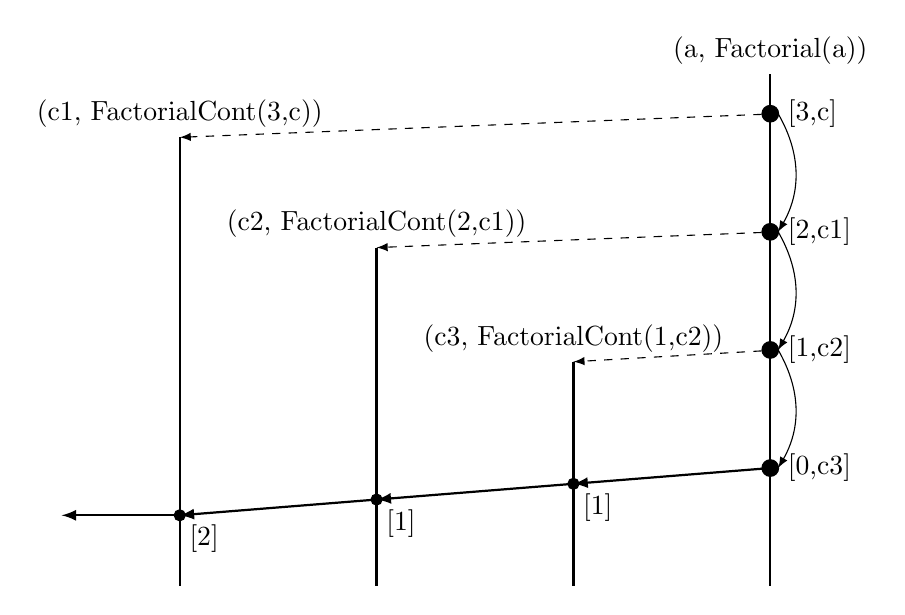
\begin{tikzpicture}
\draw[thick] (8,7) -- (8, 0.5);

\node[] (a1) at (8,7.3) {(a, Factorial(a))};

\node[align=center, right] (a1) at (8.1,6.5) {[3,c]};
\draw[fill] (8,6.5) circle (3pt);

\node[align=center, right] (a2) at (8.1,5) {[2,c1]};
\draw[fill] (8,5) circle (3pt);

\node[align=center, right] (a3) at (8.1,3.5) {[1,c2]};
\draw[fill] (8,3.5) circle (3pt);

\node[align=center, right] (a4) at (8.1,2) {[0,c3]};
\draw[fill] (8,2) circle (3pt);

\draw[-latex] (a1.west) to[bend left] (a2.west);
\draw[-latex] (a2.west) to[bend left] (a3.west);
\draw[-latex] (a3.west) to[bend left] (a4.west);

\node[] (d1) at (0.5,6.5) {(c1, FactorialCont(3,c))};
\draw[thick] (d1.south) -- (0.5, 0.5);

\node[] (c1) at (3,5.1) {(c2, FactorialCont(2,c1))};
\draw[thick] (c1.south) -- (3, 0.5);

\node[] (b1) at (5.5,3.65) {(c3, FactorialCont(1,c2))};
\draw[thick] (b1.south) -- (5.5, 0.5);


\draw[fill] (5.5,1.8) circle (2pt);
\node[align=center, right] (b2) at (5.5,1.5) {[1]};

\draw[fill] (3,1.6) circle (2pt);
\node[align=center, right] (c2) at (3,1.3) {[1]};

\draw[fill] (0.5,1.4) circle (2pt);
\node[align=center, right] (d2) at (0.5,1.1) {[2]};

\draw[-latex, thick] (8,2)  -- (5.5,1.8);
\draw[-latex, thick] (5.5,1.8) -- (3,1.6);
\draw[-latex, thick] (3,1.6) -- (0.5,1.4);
\draw[-latex, thick] (0.5,1.4) -- (-1,1.4);

\draw[-latex, black, dashed] (a1.west) -- (d1.south);
\draw[-latex, black, dashed] (a2.west) -- (c1.south);
\draw[-latex, black, dashed] (a3.west) -- (b1.south);

\end{tikzpicture}
\caption{El diagrama ilustra el cálculo del factorial de 3, todo el resultado es
enviado al actor \textit{c}. Las lineas en punto indican la creación de un actor.}
\end{figure}


\section{CSP y actores}
Para empezar a describir como se modeló en CSP, primero es importante hacer
referencia a que se utilizó CSPm, que combina los operadores de CSP
originalmente propuesto por Hoare, y un lenguage funcional.

En el proceso de traducción de SAL a CSPm, fue necesario construir un pequeño
\textit{runtime} para emular como los actores corren. Recordemos que la
naturaleza de CSP es sincrona y los actores no lo son. Fue necesario
concretamente desacoplar el pedido de creación de los actores de la creación
misma, tambien el envio y la recepción de mensajes. 

\subsection{Creación de nuevos actores}

Para desacoplar la creación de actores se utilizan dos abstracciones,
\textbf{ActorID} y un par de canales que comunican, la intención de crear un
actor por parte de otro, y el momento en el que este actor es activado.Se
menciona activación y creción, dado que CSPm necesita conocer la red completa
de procesos involucrados al comienzo de la simulación fue necesario simular la creación.

Para definir \textbf{ActorID} utilizaremos tipos alegbraicos parecidos a los de haskell.

\[
datatype\ ActorID = Factorial.\{1\} | FactorialWorker.\{1,2,3\} | Main.\{1\}
\]

Este tipo introduce y nombra cada uno de los actores que van ser utilizados. Es
decir, no solo incluye el nombre, sino que la cantidad. Para esto se utiliza la
notacíon que se ve entre llaves, en este caso vamos a contar con un actor del
tipo \textbf{Factorial}, tres dle tipo \textbf{FactorialWorker} y uno más del
tipo \textbf{Main}.


\[
channel\ CreateAsk:ActorID.(Value, Value)\\
channel\ Create:ActorID.(Value, Value)
\]

Estos dos canales de CSP, son los encargados de desacoplar la creación,
\textbf{Value} es un tipo de datos representa los valores que pueden ser pasado
tanto en la creación de actores como en el envio de mensajes. Los valores a
utilizar son enteros, \textbf{ActorID} o \textbf{ATOMS}, este último se usa para
denominar un tipo de cadena de caracteres inmutable.

Ademas del actor que envia la intención de crear, y el que lo recibe finalmente,
existe un proceso auxiliar que comunica estas dos accciones.

\[
CreateAsk!FactorialWorker.1?m \then Create.FactorialWorker.1!m \then \Stop\\
CreateAsk!FactorialWorker.2?m \then Create.FactorialWorker.2!m \then \Stop\\
CreateAsk!FactorialWorker.3?m \then Create.FactorialWorker.3!m \then \Stop
\]


Este proceso simplemente espera a sincronizar con un evento de tipo
\textit{CreateAsk} y emite un evento de tipo \textit{Create}.
En la semantica de CSP cuando utilizamos \textbf{`?'} estamos esperando un valor
por un canal, si utlizamos \textbf{`!'} estamos enviando.

En el ejemplo se puede ver que se envia el valor $FactorialWorker.1$ a quien esté
dispuesto a sincronizar, y se recepciona $m$ que equivale a la tupla de valores
antes vista. Luego se espera a sincronizar con $Create.FactorialWorker.1$ a
quien se le envía el valor de $m$.

Esto no desacopla la creción que sino que, al mismo tiempo, La asignación de un
único nombre al actor. En este caso es el valor que se envía mediante
$CreateAsk$.

\subsection{Envio de mensajes}
Para desacoplar el envío de mensajes utilizamos una estructura intermedia que
actua de \textit{mailbox}, para comunicarase con esta estructura existen dos canales.

\[
channel\ CommSend:ActorID.(VALUE, VALUE)\\
channel\ CommRecv:ActorID.(VALUE, VALUE)
\]

Un actor se bloquea esperando en $CommRecv$, cuando una nueva comunicación está
dispuesta a ser sincronizada, desde el mailbox hacia el actor, se procesa.
Generalmente la primera acción de cualquier actor es esperar la llegada de un
menasaje.

Un \textit{mailbox} puede guardar más de un mensaje en su interior. Esto
introduce un tipo de no determinismo, un actor puede sincronizar con cualquiera
de los mensajes disponibles en su \textit{mailbox}.

Por cada actor creado, existe un \textit{mailbox} con el mismo \textbf{ActorId}
asociado a este. 

\subsection{Definición de comportamientos}
La definición de comportamientos es quien utiliza las dos abstracciónes antes
mencionadas.
Para mostrar como funciona, se utilizará un ejemplo simple, un actor que cuando
es creado recive un parametro \textbf{ActorId}, luego se queda esperando un
mensaje, cuanado lo recive, utiliza el valor entero que recepciona, y lo
incrementa en uno y lo envia a la referencía del actor que recibió en el
momento de creación.

\[
g = Create!G.1?(a1, None) \then g_{running}(G.1, a1) \\ 
g_{running}(self, ACTOR.client) = \\
\quad CommRecv.self!(INT.v, None) \then \\
\quad CommSend.client!(add(v, SI.1), None) \then \\ 
\quad g_{running}(self, ACTOR.client) \\
\]

Desarmando el ejemplo, una vez recibido el mensaje $Create!G.1?(a1, None)$,
podemos decir que el actor está \textit{Corriendo}. Para eso utilizamos la
funcíon $g_{running}$. Cuando un comportamiento reacciona a un mensaje, tiene que
definir el comportamiento de reemplazo, en este caso puede ser el mismo
comportamiento que antes. Para esto tambien se utliza esta función, esto se
puede ver en la última linea del ejemplo, esta tambien podría haber sido $\Stop$,
si no hubiera un nuevo comportamiento (botton behaviour).

$CommRecv$ espera en el mailbox \textit{self} que el mailbox que es el mailbox
propio al actor, cuando recibe el mesaje $CommSend.client$ Envia un evento al
mailbox de $client$ con la tupla $(add(v, SI.1), None)$. Como utilizamos una
represantación mas pequeña de los enteros para evitar //TODO: PROBLEMAS CON LOS
ENTEROS GRANDES. El proceso de \textit{mailbox} estará esperando sincronizar
la recepción con el evento $CommSend$ y lo guardará y esperara que el actor esté
disponible para sincronizar el evento $CommRecv$ que efectuará la entrega.

\subsection{Ejemplo: cálculo de factorial en CSPm}
Se utilizará el mismo ejemplo del factorial antes visto en sal \textbf{SAL},
está compuesto por dos comportamientos $Factorial$ y $FactorialWorker$.

\subsubsection*{Comporamiento de Factorial}

La primer parte del factorial es una suerte de preludio que conecta un actor que
no está corriendo, o no fue creado con uno que fue creado. 

\[
factorial = Create.Factorial.1?(None, None) \then factorial_{running}(Factorial.1) 
\]

En el caso de la formula anterior, espera a sincronizar con sun mensaje de
creación con los parametros correspondientes. Esto no solamente simula la
creación, sino que al mismo tiempo se asigna el mailbox con nombre $Factorial.1$
al actor que está corriendo.
En el caso del comportamiento concreto hace referencia a $self$ como nombre de
su propio mailbox, en este caso se necesita instanciar un solo actor de tipo
$Factorial$ mas adelante veremos como funciona esto cuando se requieren varios
actores de un tipo.

\[
factorial_{running}(self) = CommRecv?self.(ACTOR.mailboxClient, INT.k) \then     \\
\textbf{if} (eq(k,SI.0)) \\
\quad  then \\
\quad \quad CommSend!mailboxClient.(INT.SI.1, None) \then factorialRunning(self) \\
\quad \textbf{else} \\
\quad \quad \textbf{let} \\
\quad \quad \quad newK = sub(k, SI.1) \\
\quad \quad \textbf{within} \\
\quad \quad \quad CreateAsk?FactorialWorker.pid!(INT.k, ACTOR.mailboxClient) \then \\
\quad \quad \quad CommSend!self.(ACTOR.FactorialWorker.pid, INT.newK)  \then \\
\quad \quad \quad factorial_{running}(self)
\]

El comportamiento del fragmento de código anterior, es exactamente lo mismo que
hace el código antes visto en SAL. Cuando recibe un mensaje, este contiene dos
parametros: el mailbox del cliente, y un entero K. Si este entero K fuera 0,
enviamos el valor uno al mailbox del cliente.
En caso contrario, crea un actor de tipo \textbf{FactorialWorker} y asigna su
mailbox a \textit{FactorialWorker.pid} le envia a este un mensaje con un valor
\textit{newK} que es basicamete $k-1$.
En ambos caso el comportamiento de reemplazo para el mailbox acutal, es el mismo
que antes.

\subsubsection*{Comporamiento de Worker}

\[
factorialWorker  = \Interleave_{x : \{|FactorialWorker|\}} Create!x?(k, mailboxClient) \\ 
\quad \then factorialWorker_{running}(x, k, mailboxClient)
\]


\[
factorialWorker_{running}(self, INT.k, ACTOR.mailboxClient) = \\
CommRecv.self?(INT.n, None) \then \\
\quad \textbf{let} \\
\quad \quad val = mult(n, k) \\
\quad \textbf{within} \\
\quad \quad CommSend.mailboxClient!(INT.val, None) \then \\
\quad \Stop
\]


A diferencia del actor anterior, ya que en este caso necesitamos mas de un actor
del tipo \textbf{FactorialWorker}, en la primer linea puede verse que se
comienzan en paralelo utlizando el operador de interliving de $CSPm$ tantos
procesos como elementos existan \textbf{FactorialWorker}. //TODO: INCLUIR UN
EJEMPLO DE LA NOTACIÓN.

Utilziando esta notación el tipo de datos \textbf{ActorID}, tiene dos
responsabilidades: nombrar los actores y enumerarlos. Recordemos que es
necesario conocer la cantidad total de procesos que va a tener un red de $CSP$
antes de comenzar la simulación.

Este comportamiento es muy simple, en el momento de creación recibe dos
parametros, un entero k y un mailbox. En el momento de recibir un mensaje, este
toma el valor enviado en este mensaje lo multiplica y se lo envía a el mailbox
que recibio originalmente en el momento de creación.

No tiene comportamiento de reemplazo.

\subsection{Ejemplo: Una pila en SAL}

Introducir el código en sal, y explicar como funciona.

\subsection{Ejemplo: Una pila en CSPm}

Introducir el código en CSPm equivalente y explicar las particularidades.

\subsection{Ejemplo: Un cliente-servidor de chat en SAL}

Introducir el código en sal, y explicar como funciona.

\subsection{Ejemplo: Un cliente-servidor de chat en CSPm}

Introducir el código en CSPm equivalente y explicar las particularidades.

\subsection{Traduciendo de SAL a CSPm}

Mostra la función que traduce de SAL a CSPm



TODO: Definir \textbf{translateExp}

La clase \textbf{Cmnd} con elementos de tipo S está dada por:

\begin{verbatim}
S :== S_1 ; S_2 | if b then S_1 else S_2 | send [e1, .., e_i] to a | become new
E(e_1, .. ,e_i) | let a_1 = new E_1(e_1,..,e_i) and ... a_j = new
E_1(e_1,..,e_i) { S } 
\end{verbatim}

definimos la funcion \textbf{translateCmd} de la siguiente forma:

\begin{verbatim}
translateCmd (S_1 S_2) = translateCmd(S_1) -> translateCmd(S_2)
\end{verbatim}


\begin{verbatim}
translateCmd(if b then S_1 else S_2) = 
   if (translateExp(b)) then
       translateCmd(S_1) else 
       translateCmd(S_2)
\end{verbatim}

\begin{verbatim}
translateCmd(send[e_1, ..., e_i] to a) = CommSend.a.
         (translateExp(e_1), ..., 
          translateExp(e_i)) 
\end{verbatim}

\begin{verbatim}
translateCmd(become new Beh(e_1, ..., e_n)) = runningBeh(self, e_1, ..., e_n)
\end{verbatim}

newEnv es el resultado de agregar a el entorno de las variables de mailbox $a_1
= E_1.pid_1$ .. $a_n = E_n.pid_n$
\begin{verbatim}
translateCmd(let a_1 = new E_1(e_1, ..., e_j) and 
         ... and a_n = new E_N(e_1, ..., e_j) { S } = 

CreateAsk?E_1.pid_1!(translateExp(e_1), ...,translateExp(e_j)) ->
CreateAsk?E_N.pid_n!(translateExp(e_1), ...,translateExp(e_j)) ->
translateCmd(S, newEnv)
\end{verbatim}


La clase \textbf{Beha} con elementos de tipo S está dada por:

\begin{verbatim}
def behName(a_1 .. a_i)[n_1 ... n_j]
  S
end def
\end{verbatim}

Tendria como equivalente en CSP:

\begin{verbatim}

behName = ||| actorId : {|BehName|} @ Create.actorId?(a_1, ..., a_i) ->
behNameRunning(actorId, a_1, .., a_n)

behNameRunning(self, a_1, .., a_n) = CommRecv.self(n_1 ... n_j) -> translateCmd(S)

\end{verbatim}

--- Agregar case? ---


\bibliography{references}{}
\bibliographystyle{plain}
\end{document}

